\documentclass[conference]{IEEEtran}
\usepackage[T1]{fontenc} % to have good hyphenation
\usepackage[utf8]{inputenc} % accented characters in input
\usepackage[portuguese]{babel}
\usepackage{spverbatim}
\usepackage{float}
\usepackage{listings}
\usepackage{multirow}
\IEEEoverridecommandlockouts
% The preceding line is only needed to identify funding in the first footnote. If that is unneeded, please comment it out.
\usepackage{cite}
\usepackage{amsmath,amssymb,amsfonts}
\usepackage{algorithmic}
\usepackage{graphicx}
\usepackage{textcomp}
\usepackage{xcolor}
\def\BibTeX{{\rm B\kern-.05em{\sc i\kern-.025em b}\kern-.08em
    T\kern-.1667em\lower.7ex\hbox{E}\kern-.125emX}}
\begin{document}

\title{Paper Title*\\
{\footnotesize \textsuperscript{*}}
\thanks{}
}

\author{\IEEEauthorblockN{1\textsuperscript{st} João Victor F. Machado}
\IEEEauthorblockA{\textit{ITAU XX} \\
joao.freitas-machado@itau-unibanco.com.br}
\and
\IEEEauthorblockN{2\textsuperscript{nd} Filipe A. N. Verri}
\IEEEauthorblockA{\textit{Instituto Tecnológico de Aeronáutica (ITA)} \\
 verri@ita.br\\
}

}

\maketitle

\begin{abstract}
This document is a model and instructions for \LaTeX.
This and the IEEEtran.cls file define the components of your paper [title, text, heads, etc.]. *CRITICAL: Do Not Use Symbols, Special Characters, Footnotes, 
or Math in Paper Title or Abstract.
\end{abstract}

\begin{IEEEkeywords}
component, formatting, style, styling, insert
\end{IEEEkeywords}

%%%%%%%%%%%%%%%%%%%%%%%%%%%%%%%%%%%%%%%%%%%%%%
%%%%%%%%%%%%%%%%%%%%%%%%%%%%%%%%%%%%%%%%%%%%%%
%%%%%%%%%%%%%%%%%%%%%%%%%%%%%%%%%%%%%%%%%%%%%%
%%%%%%%%%%%%%%%%%%%%%%%%%%%%%%%%%%%%%%%%%%%%%%
\section{Introdução}
  A era da coleta de informações  em larga escala conduziu ao que hoje denominamos por Big Data\cite{b11} e permitiu, por meio de algoritmos e aumento substancial da capacidade de processamento das máquinas , ao que denominamos por aprendizado de máquina, que por meio dos dados identifica padrões e aprende a reproduzi-los. O problema na procura por padrões em dados não é recente e na década de 50, Alan Turing propôs um teste da capacidade de uma máquina de exibir um comportamento inteligente equivalente ou indistinguível do comportamento de um humano.
  
 \begin{figure}[htbp]
\centerline{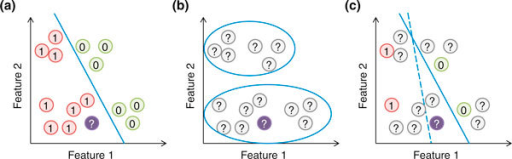
\includegraphics[scale=0.5]{imagem_aprendizado.png}}
\caption{Exemplo de tipo de aprendizado de máquina.}
\label{fig1}
\end{figure}

  A forma desse aprendizado pode ser conduzido por 3 formas distintas\cite{b12}, o primeiro é o aprendizado supervisionado como podemos ver em \ref{fig1}(a), em que temos as características de uma determinada observação (variáveis explicativas ou features) e o que denominamos por variável resposta, que é o que a máquina tem como objetivo aprender, representado pelos círculos em que cada cor representa uma classe. O lado oposto desse tipo de aprendizado é o caso de aprendizado não supervisionado representado por \ref{fig1}(b), em que temos uma coleção de dados e não temos necessariamente uma variável resposta e permite que o próprio sistema desenvolva suas conclusões por similaridades.
  
  No meio termo entre o Aprendizado Supervisionado e Não supervisionado, temos o caso do aprendizado Semi-Supervisionado \ref{fig1}(c), em que existe uma variável objetivo mas existem rótulos que não estão preenchidos, na maioria dos casos esse problema ocorre quando o problema de preenchimento é manual e não de forma automática, e o processo de preenchimento é longo e caro.
  
  No campo de Aprendizado Semi-supervisionado diversas técnicas vem sendo desenvolvidas devido a crescente dos problemas nessa área. Entre as áreas  NIGAM et al. (2000) \cite{b1}  no campo de modelos generativos, aplicou o algoritmo EM para a tarefa de classificação de texto. Wagstaff et al\cite{b14} utilizou-se de técnicas de clusterização baseada em médias, incluen-se trabalhos com técnicas baseadas em SVM(Vapnik;1999\cite{b2}) e co treinamento(Blum and Mitchell, 1998\cite{b3}). Outra solução é o  de auto-aprendizagem que foram pioneiras no problema, em que o modelo com rótulos é utilizado para classificar os dados sem rótulos.
  
  Dentre as áreas, as que se baseiam na teoria de grafos  recebem uma atenção especial pela capacidade de aprendizagem, seja a partir de uma informação local, seja ela global. Nesse caso, cada instância de dados é representada por um vértice e está vinculada para outros vértices de acordo com uma regra de afinidade predefinida. Os rótulos se propagam para todo o grafo usando um determinado otimização heurística. Otimização heurística é um algoritmo proposto para resolver determinado problema de forma mais veloz e eficiente, ou quando métodos clássicos não conseguem encontrar uma solução exata, geralmente este tipo de método reduz %%%%%%% revisar.  %%%%%%%%%%%%%%%%%%%%%%%
  precisão á velocidade. 
  
  A teoria dos grafos, nos últimos três séculos se tornou a principal linguagem matemática para descrever as propriedades das redes ou networks(Harary 1995\cite{b4}). Em sua forma mais simples, uma rede é
nada mais que um conjunto de elementos discretos (os vértices) e um conjunto de conexões (as arestas) que vinculam os elementos, geralmente de forma de pares. Os elementos e suas conexões podem ser quase tudo - pessoas e amizades (Rapoport e Horvath 1961\cite{b5}), computadores e linhas de comunicação (Faloutsos et al. 1999\cite{b6}),substâncias químicas e reações (Jeong et al. 2000; Wagner e Fell 2001) e etc. Uma extensão das redes é o que denominamos por redes complexas ou Complex networks, são grafos de grande escala com topologia não trivial. Essas redes introduzem uma ferramenta poderosa para descrever a interação de topologia, estrutura e dinâmica do que denominamos por sistemas complexos. Um sistema complexo é um sistema composto de muitos componentes que podem interagir entre si. Como exemplos de sistemas complexos podemos citar o clima global da Terra, organismos, o cérebro humano, infra-estrutura como rede elétrica, sistemas de transporte ou comunicação, e etc. 
As redes(networks) geralmente descrevem as fontes de complexidade em sistemas complexos. Estudar sistemas complexos como redes, portanto, permite muitas aplicações úteis da teoria dos grafos e da ciência de redes.

No sentido de estudos de sistemas complexos utilizando-se da teoria de grafos, Verri et al.(2018)\cite{b7}, utilizando-se de um mecanismo de aprendizado de redes complexas, denominado por disputa de partícula, propôs um modelo de aprendizagem semi-supervisionado que emprega um sistema dinâmico de vértice-aresta que utiliza-se da característica de propagação da classe em redes complexas, Nesse sistema dinâmico, ``Edge Domination System (EDS)'', as partículas competem por arestas em uma rede. As sub-redes são geradas com as arestas agrupadas por dominância de classe. Aqui, nós chamamos cada sub-rede como um desdobramento. O modelo de aprendizagem emprega os desdobramentos para classificar dados não rotulados. O modelo proposto oferece desempenho satisfatórios em problemas de aprendizagem semi-supervisionados em conjunto de dados artificiais e reais.


Nesse trabalho, implementamos o sistema dinâmico, ``Edge Domination System'', utilizando-se um sistema de computação em paralelo. Sistemas dinâmicos em grafos, permitem a computação em paralelo e tem sido bastante utilizada nos dados em redes, por exemplo uma gama de novos grafos em paralelos distribuídos em grande escala frameworks (por exemplo, Pregel\cite{b10}, PowerGraph\cite{b11} etc) tem emergido. Cada estrutura introduz uma nova abstração de programação que permite aos usuários descreverem compactamente algoritmos em grafos (por exemplo, PageRank, Propagação de Crença, etc..) e um tempo de execução correspondente ágil que executa eficientemente estes algoritmos em multicore. Esses sistemas paralelos de dados, como MapReduce e Spark \cite{b9}, são projetados para processamento de dados escalável e são bem adequado para a tarefa de construção de grafos (ETL). Ao explorar
paralelismo de dados, estes sistemas são altamente escaláveis e suportam uma gama de estratégias de tolerância a falhas. Sistemas mais recentes como o Spark permite até mesmo o processamento de dados interativo. 
%%%%%%%%%%%%%%%%%%%%% explicar motivaçao e como esta separado o trabalho

  
\section{Descrição do modelo}

Nesta seção introduziremos de forma breve o modelo de sistema dinâmico introduzindo o conceito de sistema de competição de partículas e em seguida expondo a forma matemática do modelo.
% ...

\subsection{O sistema de competição de partículas}

O modelo de Sistema de Dominação de Aresta modela uma competição de partículas em um processo de rede complexa. Partículas competem pela dominação de arestas da rede. A rede é um grafo simples, sem peso nas arestas, e não direcionado $G =(\mathcal{V} , E)$, onde $\mathcal{V}=\{R,NR\}$ é o conjunto de vértices, $R = \{v_{1},v_{2},...,v_{l}\}$ os vértices que estão rotulados e $NR= \{v_{l+1},..,v_{l+r}\}$ sendo os vértices não-rotulados. Cada vértice rotulado pertencente a $R$ tem label $y_{i}$ pertencente ao intervalo $\{1,...,C\}$, O número de classes C é maior do que 1. A aresta entre $v_{i}$ e $v_{j}$ nós denotamos por $(i,j)$. O número de vértices totais é $(R + NR)$, com a suposição de que a concentração de dados rotulados é menor do que a de não rotulados, ou seja $R<NR$. A rede pode ser representada pela matriz de adjacência $A = (a_{ij})$, temos que a matriz A é simétrica $a_{ij}=a_{ji}$.

As Partículas caminham aleatoriamente do vértice ao vértice, carregando um rótulo fixo. Para uma partícula carregando rótulo C (classe), qualquer partícula / vértice
de um rótulo diferente de C é uma partícula / vértice rival. A borda conta o número de partículas que passam por ela, separadamente por cada etiqueta. O rótulo com a maior contagem é o rótulo que domina essa borda. Neste sistema, uma variável denotada por número de partículas pode ser gerado ou removido do sistema. Uma partícula em qualquer vértice escolhe o próximo vértice com igual probabilidade entre os vizinhos do vértice corrente. Essa variável pode ser gerada ou removida de três formas distintas: \textbf{caminhando}, uma partícula em qualquer vértice escolhe o próximo vértice com igual probabilidade entre os vizinhos do vértice corrente. \textbf{Absorção}, a classe dominante no vértice determina se a partícula vai para o vértice ou se desaparece do sistema. \textbf{Geração},  um vértice rotulado gera partículas de acordo com seu grau e de acordo com o número de partículas no sistema. A figura \ref{fig2} retrata como funciona o sistema de competição de partículas.


\begin{figure}[htbp]
\centerline{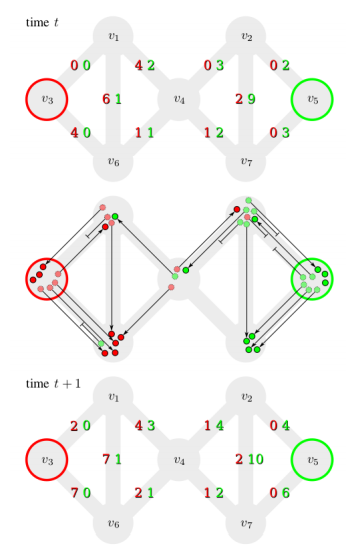
\includegraphics[scale=0.5]{imagem_2.PNG}}
\caption{Exemplo retirado de Verri et al.(2018).
Ilustração de uma iteração da evolução do sistema. A rede consiste de 7 vértices e 10 arestas; cada cor representa um rótulo de uma partícula ou uma fonte. A primeira e a terceira redes descrevem a dominação cumulativa antes e depois da iteração. A dominação cumulativa é o número de visitas de partículas a uma borda desde o estado inicial. Na segunda rede,
as partículas são representadas em pequenos círculos. Partículas ativas no tempo t são descritas bordas destacadas, enquanto as partículas ativas no tempo t + 1 estão em borda completa}
\label{fig2}
\end{figure}

 Em nosso trabalho a versão utilizada é a forma simplificada de Verri et al(2018)\cite{b13}, em que o algoritmo proposto  consiste na simulação de um sistema dinâmico coletivo baseado na competição de partículas pela dominância de arestas, diferindo na notação alternativa($y_{i}=0,1,...,C$) para os rótulos.


\subsection{Entrada.}


Uma matriz $A = (a_{ij})$ com $i=1,...,V$ e $j=1,...,V$ tal que $a_{ij} \, \in \, \{0,1\}$, temos as seguintes propriedades : 
\\
\begin{itemize}
\item A é simétrica, ou seja, $a_{ij}$= $a_{ji}$ para todo $i,j$.

\item A diagonal da matriz A é nula, ou seja, $a_{ii} = 0 $
\item A matriz A é esparsa, $|\{(i,j):a_{ij}=1\} \ll |\{(i,j):a_{ij}=0\} $
\end{itemize}

Um vetor de classes $\vec{y}=[y_{i}], \, i=1,...,V$ tal que $y_{i} \, \in \, \{0,1,...,C\}, \, C\geq 2$ em que $y_{i}=0$ significa o dado sem label(não rotulado) e $y{i}$ resulta na classe do vértice i. 
%...

Definimos a partir de  $A$ e $\vec{y}$, os  vetores de entrada do sistema dinâmico :

\begin{equation}
   X(t) = \begin{bmatrix}
       \bold{n}^{c}(t)=[n_{i}^{c}]_{c=1,...,|V|}       \\
       N^{c}(t) = (n_{ij}^{c}(t))_{i,j=1,...,|V|}
     \end{bmatrix} 
\end{equation}

Onde $\bold{n}^{c}(t)$ é um vetor, onde cada elemento ${n}^{c}_{i}(t)$ é o número de partículas ativas pertencendo a classe (c) no tempo ($t_{i})$.  

como pré requisitos do sistemas, temos:
\begin{itemize}
    \item $\displaystyle\sum_{j:y_{j}=0}a_{ij}>0,$ para todo $i=1,...,V$, \newline
    \item $a_{ij}=0\quad$ se $y_{i},y{j}\neq0$ e $y_{i}\neq y_{j}$, \newline
    
    \item $n_{i}^{c}=0$ se $y_{i} \neq 0$ e $y_{i} \neq c$, \newline
    
    \item  $n_{i}^{c}(0)>0$  \newline
    
    \item $\displaystyle\sum_{i}n_{i}^{c}(0)=1$ , e  \newline
\end{itemize}
%%%%%%%%%%%%%%%%%%%%%% N(t) ???


\begin{equation}
n_{ij}^{c}(0) =
           \begin{cases}
             0 \quad se \, y_{i} \neq c\\
            0 \quad se \, y_{j} \neq c\\
            1 \quad caso \, contrário
        \end{cases}
\end{equation}


\subsection{Variáveis Auxiliares.}
 Aqui temos variáveis que durante a evolução do sistema permanecem inalteradas.
 
Para todo $i=1,...,V$:
\begin{equation}
    k_{i}=\displaystyle\sum_{j} a_{ij}
\end{equation}
 Para todo $i=1,...,V$ e $c=1,..,C$:
 
 \begin{equation}
p_{i}^{c} =
           \begin{cases}
             0 \quad se \, y_{i} \neq c  \\
            \frac{k_{i}}{\sum_{j:y_{j} \neq c}k_{j}}  \quad caso  \, contrário \\
        \end{cases}
\end{equation}
 \\
\subsection{Evolução do Sistema}
 \begin{equation}
\phi =
           \begin{cases}
            \vec{n^{c}}(t+1)= \vec{n}^{c}(t) \times P^{c}(X(t)) + \vec{g}^{c}(X(t)) \\
            N^{c}(t+1) = diag \, \vec{n}^{c}(t) \times P^{c}(X(t)) \\
        \end{cases}
\end{equation}

\begin{equation}
    p^{c}_{ij}(X(t)) = \frac{a_{ij}}{k_{i}}
    \frac{n_{ij}^{c}(t)+ n_{ji}^{c}(t)}{\sum^{C}_{q=1}n_{ij}^{q}(t) + n_{ji}^{q}(t)}
\end{equation}
\begin{equation}
    g_{i}^{c}(X(t)) = p_{i}^{c} \max(0,1-\vec{1} \cdot \vec{n}^{c}(t))
\end{equation}

\subsection{Saída}
\begin{equation}
    \lim\limits_{x \to \infty} X(t)
\end{equation}


\section{Map reduce e Pyspark}

O sistema foi implementado em Pyspark, a API Spark Python (PySpark) expande o modelo de programação do Spark ao Python, no PySpark, os RDDs (Resilient Distributed Dataset)\cite{b10} suportam os mesmos métodos que seus correspondentes Scala, mas usam funções Python e retornam tipos de objeto Python. Funções curtas podem ser passadas para métodos RDD usando a sintaxe lambda do Python. Em nosso trabalho  foi utilizado a classe \texttt{pyspark.mllib.linalg.distributed} que implementa no pyspark um módulo para álgebra linear distribuída, o primeiro passo é transformar nosso dataframe em uma matriz distribuída, a partir do BlockMatrix que é uma matriz distribuída apoiada por um RDD de MatrixBlocks, abaixo um exemplo de código para essa transformação:

\lstset{language=Python}
\lstset{frame=lines}
\lstset{caption={Exemplo de função Map para  }  }
\lstset{label={lst:code_direct}}
\lstset{basicstyle=\footnotesize}
\begin{lstlisting}
from pyspark.mllib.linalg import *
from pyspark.mllib.linalg.distributed import *

def as_block_matrix(rdd, rowsPerBlock=1024,
    colsPerBlock=1024):
    return 
    IndexedRowMatrix(
        rdd.zipWithIndex().map(lambda xi:
        IndexedRow(xi[1], xi[0]))
    ).toBlockMatrix(rowsPerBlock, colsPerBlock)
  
\end{lstlisting}

A função acima utiliza-se por base o BlockMatrix, este suporta métodos como adicionar e multiplicar com outro BlockMatrix. Além disso O BlockMatrix também possui uma função auxiliar que pode ser usada para verificar se o BlockMatrix está configurado corretamente. A função \texttt{add}, função de adição de matrizes, obriga que as matrizes devem ter o mesmo tamanho e valores correspondentes de rowsPerBlock e colsPerBlock. Se um dos blocos de sub matriz que estão sendo adicionados for uma matriz esparsa, o bloco de submatriz resultante também será uma matriz esparsa. Outros métodos que estão implementados e foram utilizados é o método transpose, que como resultado é a transposta da matriz.

Abaixo podemos verificar a implementação do algoritmo utilizando a função \texttt{as\_block\_matrix} para transformar as matrizes Python em matrizes distribuídas, além dos métodos \texttt{add} e \texttt{tranpose}.

\lstset{language=Python}
\lstset{frame=lines}
\lstset{caption={Trecho do código de evolução do sistema em Spark}}
\lstset{label={lst:code_direct}}
\lstset{basicstyle=\footnotesize}
\begin{lstlisting}
max_epochs = 10   # numero de epocas
for epochs in range(max_epochs):
  NT = list()
  matrixN = as_block_matrix(sc.parallelize(N[0]))
  teste = matrixN.add(matrixN.transpose()).toLocalMatrix()
  .toArray()
  NT.append(teste)
  Ntotal = np.array(NT[0]) 
  ...

\end{lstlisting}

Em outro trecho do código com a função de multiplicação de matrizes,"multiply": 

\lstset{language=Python}
\lstset{frame=lines}
\lstset{caption={Trecho do código de evolução do sistema em Spark}}
\lstset{label={lst:code_direct}}
\lstset{basicstyle=\footnotesize}
\begin{lstlisting}
  ...
      P = as_block_matrix(sc.parallelize(W * Lambda))
      g = rho[l-1].T * (1 - sum(n[l-1]))
      N[l-1] = as_block_matrix(sc.parallelize(
               np.diag(n[l-1]))).multiply(P)
  ...

\end{lstlisting}



\section{Resultados}\label{AA}

 As redes de entrada utilizadas consistem de 128 vértices divididos em 4 classes balanceadas.  As redes foram geradas utilizando o benchmark de Girvan-Newman [1] com grau médio $z_\text{in} + z_\text{out} = 16$ e com razões $z_\text{out}/z_\text{in}$ variando conforme a Tabela \ref{tab:benchmark}.

\begin{table}[h!]
\centering
\caption{Razões $z_\text{out}/z_\text{in}$ dos benchmarks de Girvan-Newman}
\label{tab:benchmark}
\begin{tabular}{c c}
Número do benchmark & $z_{\text{out}}/z_{\text{in}}$ \\
Benchmark1 & 0.067 \\
Benchmark2 & 0.143\\
Benchmark3 & 0.231\\
Benchmark4 & 0.333  \\
Benchmark5 & 0.455  \\           
Benchmark6 & 0.6  \\ 
Benchmark7 & 0.778 \\ 
Benchmark8 & 1
\end{tabular}
\end{table}

 Abaixo podemos ver a Figura \ref{grafo_comlabel}  de um dos benchmarks com as classes todas representadas, utilizamos esses benchmarks a fim de verificar a implementação em Spark, apesar de não ser uma rede complexa estes testes suprem uma primeira verificação de implementação.
 
\begin{figure}[H]
\centerline{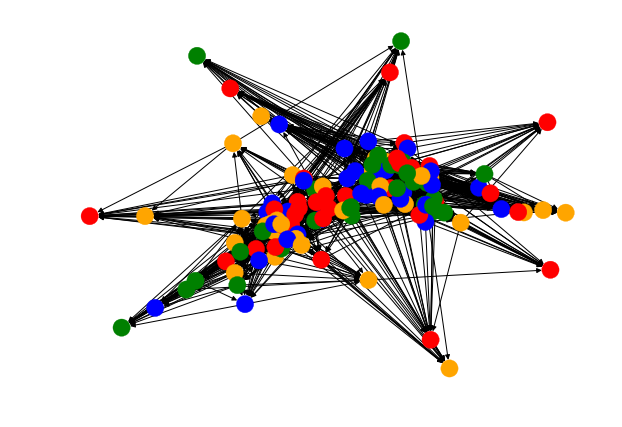
\includegraphics[scale=0.4]{grafo.png}}
\caption{base utilizada com labels correspondidos pelas cores.}
\label{grafo_comlabel}
\end{figure}

\begin{figure}[htbp]
\centerline{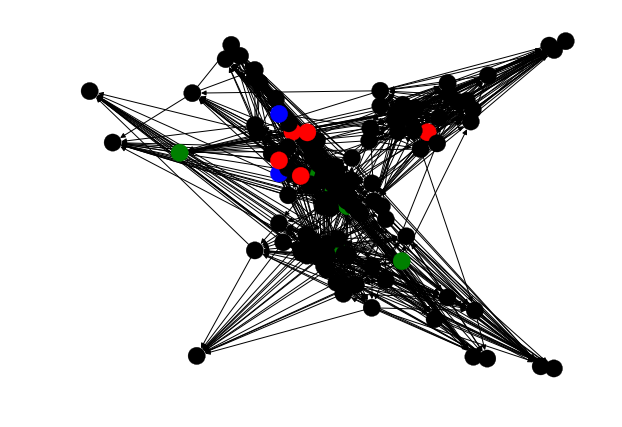
\includegraphics[scale=0.4]{download.png}}
\caption{base utilizada com 90\% dos labels mascarados(preto).}
\label{grafo_semlabel}
\end{figure}
Após os dados carregados, foi selecionado aleatoriamente 90\% dos vértices e atribuídos a estes o valor igual a 0, a Figura \ref{grafo_semlabel} representa a rede com labels(classes) mascarados, que indica que não sabemos a classe correspondente e o algoritmo deveria atribuir um valor de 1 a C  a estes vértices, após as iterações do algoritmo era verificado a acurácia:

\begin{equation}
    \frac{\sum Y_{algoritmo} == Y_{real}}{numero \, de \, vertices} \quad onde, 
\end{equation}

\begin{equation*}
    \begin{cases}
             (Y_{algoritimo} == Y_{real}) = 1 \quad se \, acerta \, classe \\
             0 \quad  caso \, contrario \\
        \end{cases}
\end{equation*}

 A tabela \ref{tab1} mostra a acurácia média obtida para cerca de 40\% dos benchmarks selecionados com diferentes razões de  $z_{\text{out}}/z_{\text{in}}$. No final os benchmarks utilizados foram: 5 amostras do \textbf{benchmark 1}, 8 amostras do \textbf{benchmark 2},5 amostras do \textbf{benchmark 3}, 5 amostras do \textbf{benchmark 4}, 12 amostras do \textbf{benchmark 6}, 6 amostras do \textbf{benchmark 7}, 7 amostras do \textbf{benchmark 8}, 4 amostras do \textbf{benchmark 5}.

\begin{table}[H]
\caption{Acurácia média obtida nos dados de benchmark com 1,3,5 e 8 épocas.}
\begin{center}
\begin{tabular}{|c|c|c|}
\hline
\textbf{Número de}&\multicolumn{2}{|c|}{\textbf{Resultados}} \\
\cline{2-4} 
\textbf{benchmarks} & \textbf{\textit{\bold{Épocas}}}& \textbf{\textit{Acuracia}} \\
\hline
\multirow{4}{}{\textbf{52} \newline} & 1& 0,842371  \\
& 3& 0,877757  \\
& 5&  0.905331 \\
& 8 &  0.936887  \\
\hline
\end{tabular}
\label{tab1}
\end{center}
\end{table}


\section{Conclusões}\label{AA}

Apesar 
 
\newpage
% 14
\begin{thebibliography}{00}
\bibitem{b11} Chen, Min, Shiwen Mao, and Yunhao Liu. "Big data: A survey." Mobile networks and applications 19.2 (2014): 171-209.
\bibitem{b12} Friedman, Jerome, Trevor Hastie, and Robert Tibshirani. The elements of statistical learning. Vol. 1. No. 10. New York, NY, USA:: Springer series in statistics, 2001.
\bibitem{b1} Nigam, Kamal, et al. "Text classification from labeled and unlabeled documents using EM." Machine learning 39.2-3 (2000): 103-134.
\bibitem{b14} K. Wagstaff, C. Cardie, S. Rogers, and S. Schroedl, “Constrained kmeans clustering with background knowledge,” in Proc. of the 18th International Conference on Machine Learning, 2001, pp. 577–584.
\bibitem{b2} Vapnik, Vladimir Naumovich. "An overview of statistical learning theory." IEEE transactions on neural networks 10.5 (1999): 988-999.
\bibitem{b3}A. Blum and T. Mitchell. Combining labeled and unlabeled data with co-training. Proceedings of the eleventh annual conference on Computational learning theory, pages 92–100, 1998.
\bibitem{b4}Hage, Per, and Frank Harary. "Eccentricity and centrality in networks." Social networks 17.1 (1995): 57-63.
\bibitem{b5}Rapoport, A. and Horvath, W. J. A study of a large sociogram. Behavioral Science 6(1961): 279-291. 
\bibitem{b6}M. Faloutsos, P. Faloutsos and C. Faloutsos, On power law 
relationships of the internet topology, ACM SIGCOMM, 1999. 
\bibitem{b7} Verri, Filipe Alves Neto et al. “Network Unfolding Map by Vertex-Edge Dynamics Modeling.” IEEE Transactions on Neural Networks and Learning Systems 29 (2018): 405-418.
%%%%%%%%%%%%%%%%%%%%%%%%%%%%%%%%%%%%%%%%%%%%%%%%%%%%%%%%%%%%%%%%%%%%%%
\bibitem{b8} Winker, P. and M. Gilli, (2004): Applications of optimization
heuristics to estimation and modelling problems. Computational
Statistics \& Data Analysis 47, 211–223.
\bibitem{b10} G. Malewicz, M. H. Austern, A. J. Bik, J. Dehnert, I. Horn,
N. Leiser, and G. Czajkowski. Pregel: a system for large-scale
graph processing. In SIGMOD, pages 135–146, 2010. 1, 4, 4.1
\bibitem{b11} J. E. Gonzalez, Y. Low, H. Gu, D. Bickson, and C. Guestrin.
Powergraph: Distributed graph-parallel computation on
natural graphs. In OSDI ’12. 1, 2, 3.1.1, 4, 4.1, 4.2
\bibitem{b9} M. Zaharia et al. Resilient distributed datasets: a fault-tolerant abstraction for in-memory cluster computing. NSDI, 2012. 1
\bibitem{b13} Verri, Filipe & Paulo Roberto Urio, and & Zhao, Liang. (2018). Advantages of Edge-Centric Collective Dynamics in Machine Learning Tasks. Journal of Applied Nonlinear Dynamics. 7. 269-285. 10.5890/JAND.2018.09.005. 
\bibitem{b10} Zaharia, Matei, et al. "Resilient distributed datasets: A fault-tolerant abstraction for in-memory cluster computing." Proceedings of the 9th USENIX conference on Networked Systems Design and Implementation. USENIX Association, 2012.
\end{thebibliography}
\vspace{12pt}


\end{document}
